\documentclass[12pt]{article}\usepackage[english]{babel}\usepackage{xcolor}\usepackage[hmargin=1in,vmargin=1in]{geometry}\usepackage{amsmath}\usepackage{unicode-math}\usepackage[round,sort,comma]{natbib}\bibliographystyle{apa}\usepackage{setspace}\usepackage{graphicx}\usepackage{caption}\usepackage{subcaption}\usepackage[colorlinks=true, allcolors=blue]{hyperref}\usepackage{float}\usepackage{booktabs}\usepackage{titlesec}\newcommand{\addperiod}[1]{#1.$\;$}\titlespacing{\section}{0pt}{\parskip}{-\parskip}\titleformat{\subsection}[runin]{\normalsize\bfseries}{\thesubsection}{1em}{\addperiod}\titleformat{\subsubsection}[runin]{\normalfont\normalsize\itshape}{\thesubsubsection}{1em}{\addperiod}\titlespacing{\subsubsection}{14pt plus 4pt minus 2pt}{0pt}{0pt plus 2pt minus 2pt}\setlength{\parindent}{1em}\makeatletter\g@addto@macro \normalsize {\setlength\abovedisplayskip{3pt plus 5pt minus 2pt}\setlength\belowdisplayskip{3pt plus 5pt minus 2pt}}\makeatother\newcommand{\comment}[1]{} \usepackage{tikz}\usetikzlibrary{positioning, shapes} \begin{document}\pagenumbering{gobble}\begin{center}{\fontsize{16}{16}\selectfont\bfseries \texttt{reproduce.work}: A framework to facilitate cross-platform computational reproducibility in scientific publishing}\\\vspace{5mm}\begin{table}[!ht]\begin{center}\begin{tabular}{c c }\shortstack{ Alex P. Miller \\USC Marshall School of Business \\alex.miller@marshall.usc.edu }\end{tabular}\end{center}\end{table}\vspace{5mm}\emph{Last updated: \today}\vspace{4mm}\hyphenpenalty=10000 \exhyphenpenalty=10000\abstract{In metascience, computational reproduction is the process of reproducing the results of a scientific paper using the data and code provided by the authors of the paper. This subject sits within the broader context of "reproducibility" in scientific  research, which has been core to the philosophy of science for decades. However, the practice of science has fallen woefully short of meeting even basic standards toward true and widespread reproducibility. In this project, we focus primarily on addressing the narrow problem of computational reproucibility. We propose a framework for facilitating computational reproducibility in scientific publishing, which we call reproduce.work. The reproducibility standards are designed to be cross-platform and to work with any programming language. We highlight the distinction between open and reproducibile practices and showcase how our software framework encourages both simultaneously. The results of this very paper can be reproduced on any machine that can execute a containerized image using the reproduce.work workflow. We conclude by discussing the potential of the framework for improving rigor and fidelity of computational science for both producers and consumers of published work.
}\\\vspace{2cm}{\scriptsize \noindent Notes: reproduce.work/v0.0.1  \raisebox{-1mm}{
\includegraphics[width=5mm]{../../nbs/img/logo.png}} }\hyphenpenalty=50 \exhyphenpenalty=50\vspace{10mm}\end{center}\newpage\doublespacing\pagenumbering{arabic}\setcounter{page}{1}

\hypertarget{introduction}{%
\section{Introduction}\label{introduction}}

An increasing number of scientists across various disciplines are calling for heightened standards of reproducibility. From biomedical research and computer science to management, psychology, and economics, the scientific community is grappling with the challenges of ensuring that published scientific work is verifiable and trustworthy. Several scholars have described the current state of affairs as an epistemological ``crisis'' in the core of science\linebreak
In its most dramatic form, high profile accusations of data fabrication have led to \verb,$,25 million dollar lawsuits and the resignation of a university presidents. 

A more mundane but pervasive manifestation of epistemological precarity is the fact that most scientific papers are not reproducible to even the lowest degree. A low percentage of published papers claim to share their data and code; of those that do, many fail to follow through or even respond to inquiries. Even when good faith efforts are made to share data and code, the vagaries of software development and the complexity of scientific code make it difficult to reproduce results across time, space, and computing environments.
\cite{dreber2019statistical}

In metascience, computational reproduction is the process of reproducing the results of a scientific paper using the data and code provided by the authors of the paper. This subject sits within the broader context of ``reproducibility'' in scientific  research, which is the idea that scientific results should be reproducible by other scientists (or anyone interested, for that matter). Concepts around reproducibility have been core to the philosophy of science for decades, but several aspects of the scientific method have been challenged by recent developments. On top of the outright fraud and misconduct that is apparently common, there are more subtle forms research malpractice and human error that are known to pervade the published scientific literature as well. Simple misunderstandings about the nature of statistical inference and the human tendency to search for patterns in data can lead to the publication of results that are not trustworthy. Further, the complexity of scientific code and restrictiveness of many data sharing agreements means that most published scientific results are not reproducible to even the lowest degree. 
Among those concerned about reproducibility on all fronts, this has led to a call for heightened standards of reproducibility in scientific research. 

To this end, we introduce a simple framework for achieving and demonstrating computational reproducibility, referred to as reproduce.work. The associated scientific development kit is designed to facilitate production of reproducible scientific computing projects by default. It features a full-featured computing environment (enabled by containerization) that is compatible with essentially any existing scientific workflow. The framework also features a suite of software that facilitates the publication of standardized computational reports with structured metadata. The framework is designed to be as simple as possible while accommodating a wide variety of scientific output. As a proof-of-concept version 0.0.1 example of this framework, the source code for this paper and the full stack containerized environment used to produce it are open source and can be found here run in any modern computing environment. 

\hypertarget{background}{%
\section{Background}\label{background}}

Replicability, in the context of the philosophy of science, metascience, and empiricism, refers to the ability of a scientific study or experiment to be independently repeated under the same conditions to verify the original results. It is a cornerstone of the scientific method, ensuring that findings are not anomalous or products of error or bias. The goal of replication is ensure that science is built on consistent and generalizable truths. The emphasis on replicability underscores the importance of transparency, rigor, and skepticism in the pursuit of knowledge; recent developments in the broader scientific community in recent years have prompted widespread introspection within about practices, methodologies, and the reliability of published findings.

While a unified concept at its core, the concept of replicability can manifest in various forms based on the specific domain or the nature of the scientific investigation. Here are how we theorize several distinct types of replicability:

\begin{itemize}
\itemsep -0.2em
\item Direct Replicability:  The most straightforward form of replication; the aim is to determine if the same results emerge under virtually identical conditions. Depending on the research methodology, this may take one of several forms:

\begin{itemize}
\itemsep -0.2em
\item Computational Replicability: This involves rerunning analyses with the original code and dataset.
\item Procedural Replicability: where researchers attempt to recreate the original study as closely as possible using the same procedures, materials, and subjects or subject pool (if applicable).
\end{itemize}
\item Conceptual Replicability/Generalizability: Rather than mirroring the original study exactly, conceptual replication involves testing the same underlying hypothesis but with different methods or procedures. This type of replication examines the robustness of the original findings and whether they can be generalized across different contexts or approaches.
\end{itemize}

While conceptual replication is obviously core to the scientific method, the focus of this project will be limited to computational replicability. We believe that computational replicability is a small but necessary first step toward a world where scientific results are verifiable. Given the low bars of existing standards in scientific practice, we beleive this project and the ideas put forward here have potential as the seed of a growing culture of scientific rigor and transparency.

\hypertarget{barriers-to-computational-reproduction}{%
\subsection{Barriers to computational reproduction}\label{barriers-to-computational-reproduction}}

We highlight several challenges to computational replication that are not necessarily unique to but are common in scientific research. 

\textbf{Lack of documentation}. Very rarely is it ever written down explicitly which code was run to generate which results in a scientific report. Even if the code is open and published by the authors, it may be complex and difficult to parse. Scientific code is often written with the intention of generating specific set of results, rather than with the intention of being read and reproduced independently. As such, the code is often not documented in a way that is easy to understand.

\textbf{Platform dependence.} Even someone is able to track down the relevant code and data, setting up the requisite computing environment to reproduce the results of a scientific report is often a non-trivial task. This is because the code that produced the results may depend on a specific version of a programming language, a specific version of a software package, or even a specific operating system.

\textbf{Code complexity}. Even if the computing environment is set up correctly, the code may be too complex to understand. This is especially true for code that is written by a researcher who principally a scientist and not a software developer. Very rarely are complex scientific analyses possible to reproduce by running a simple function or script with a single command, which means that any forms of ``reproducibility'' must be inherently flexible with respect to the computational requirements at a fundamental level. 

Allowing for arbitrary code execution is of course a hazard from a both security standpoint and a human comprehensibility standpoint. However, the next-best alternatives are have significant flaw as well. One idea might be to increase replicability by limiting the scope of the computing environment. However, if the scope of such environments becomes too narrow, it is is likely to be unable to accommodate many scientific applications. 
Another idea is to require that all code be written in a specific way that is amenable to automated verification. This is a non-starter for many reasons, not least of which is that it would require a massive shift in the way that scientific code is written. 
Current standards in most published science is that it is not even possible verify that the straightforward claims of a scientific report are reproducible, highlighting the potential for even the most basic standards to improve existing paradigms around computational reproducibility. 

\textbf{Lack of independent verification}. We put forward the following standard as the first of computational reproducibility: ``More than one person verified that the results in the published paper match the results of the code and data provided by the authors.'' This is standard, by and large, is rarely met in published science. (We believe clearing the bar of computational reproducibility may open up conversations of higher order, particularly around smarter ways to think about and operationalize independence.)

\textbf{Data availability}. Especially true for projects that rely on data collected from human participants, such data which may be subject to privacy concerns or other legal restrictions. Other reasons of propietary interest may also prevent the open sharing of data.

The last of these challenges will always remain relevant to some degree. However, this project is based on notion that the first four challenges are all amenable to software solutions to some degree. The purpose of this project is to develop a framework for computational reproducibility that is designed to overcome the challenges of poor documentation, platform dependence, and code complexity, and lack of verification. 

\hypertarget{related-projects}{%
\subsection{Related projects}\label{related-projects}}

\hypertarget{existing-environments-for-scientific-publishing}{%
\subsubsection{Existing environments for scientific publishing}\label{existing-environments-for-scientific-publishing}}

There exist a number of projects with similar aims to this one. We highlight the \href{https://jupyter.org/}{Jupyter} ecosystem --- including 
the \href{https://jupyterbook.org/en/stable/content/myst.html}{MyST Markdown} and \href{https://nbdev.fast.ai/}{nbdev} projects that both facilitate well-documented scientific software. The \href{https://rstudio.com/}{RStudio} and 
 \href{https://rmarkdown.rstudio.com/}{RMarkdown} computing environments are also widely used tools in statistical computing that have features that encourage the alignment of scientific computing and publishing. (also see \href{https://mine-cetinkaya-rundel.github.io/improve-repro-workflow-reproducibilitea-2020/}{example 1}) These projects are designed to facilitate the production of scientific reports that are both human-readable and computationally reproducible. However, these projects have some restrictions with respect to the software they are able to execute and, further, they have no mechanism or standards for verifying that the results reported in the published document are indeed reproducible. This is not a criticism, by any means; the reproduce.work project builds on these concepts but with objectives that are optimized for a specific vision of computational reproducibility. 

The reality, however, is that very few scientists have a reproducible ``environment'' in any meaningful sense of that word from the perspective of scientific computing. Most scientists use a variety of software packages and programming languages to conduct their research. They may copy and paste data between applications, such as R or Stata or MATLAB, and they may use a variety of software platforms to compose their reports. Overleaf is a popular SaaS {\LaTeX}   engine; Google Docs and Microsoft Word are a popular word processors. As such, the default environment is the ad hoc environment, which is to say that the default environment for most published scientists is no environment at all.

\hypertarget{difference-between-open-science-and-reproducible-science}{%
\subsubsection{Difference between open science and reproducible science}\label{difference-between-open-science-and-reproducible-science}}

There do exist efforts around ``open science'', which are closely related but distinct from reproducible science. See \href{https://osf.io/tvyxz/}{OSF}, for example. Note however the important distinction --- which we wish to highlight as a core observation of this project --- that reproducible science and open science are different objectives.

As mentioned above, a reproducible project is one for which at least one independent party has verified that the stated results match the actual results of the code and data provided by the authors. It is in principle quite easy to publish an ``open'' science project without clearing this bar. For example, one could publish a project with open data and code, but the code could be incorrect or the data could be manipulated. (It is also possible, in principle, for there to be reproducible projects that are not open, or selectively open depending on the access preferences of the publishing authors.)
This is not to say that open science is not a worthy goal; it is. However, we believe that reproducible science is a different objective and one that is also worth aiming for.

Given that it is no panacea for the problem of error and fraud, it worth asking whether the benefits of reproducible science are worth the effort. This project is trying to loewr the efforts required to make the calculus more favorable for reproducibility as a default standard in relevent sectors of scientific publishing. 
Even in the worst-case scenarios, where a researcher is attempting to commit fraud or deception, we believe a standardized reproducibility framework, combined with open science, can offer benefits for the aims of science as a whole. These include:

\begin{itemize}
\itemsep -0.2em
\item Traceability: Even if someone tries to abuse the system, the transparent nature of the framework ensures that their actions can be traced back and audited.
\item Standardized Inspection: Since everyone adheres to the same standard, it becomes easier to inspect, review, and identify anomalies.
\item Flexibility: The modular nature of the design means it can be adapted or updated to counter new threats or abuses as they emerge.
\end{itemize}


\begin{figure}[h]
\centering
\caption{Different models of computation and composition.}
\label{fig:comp}
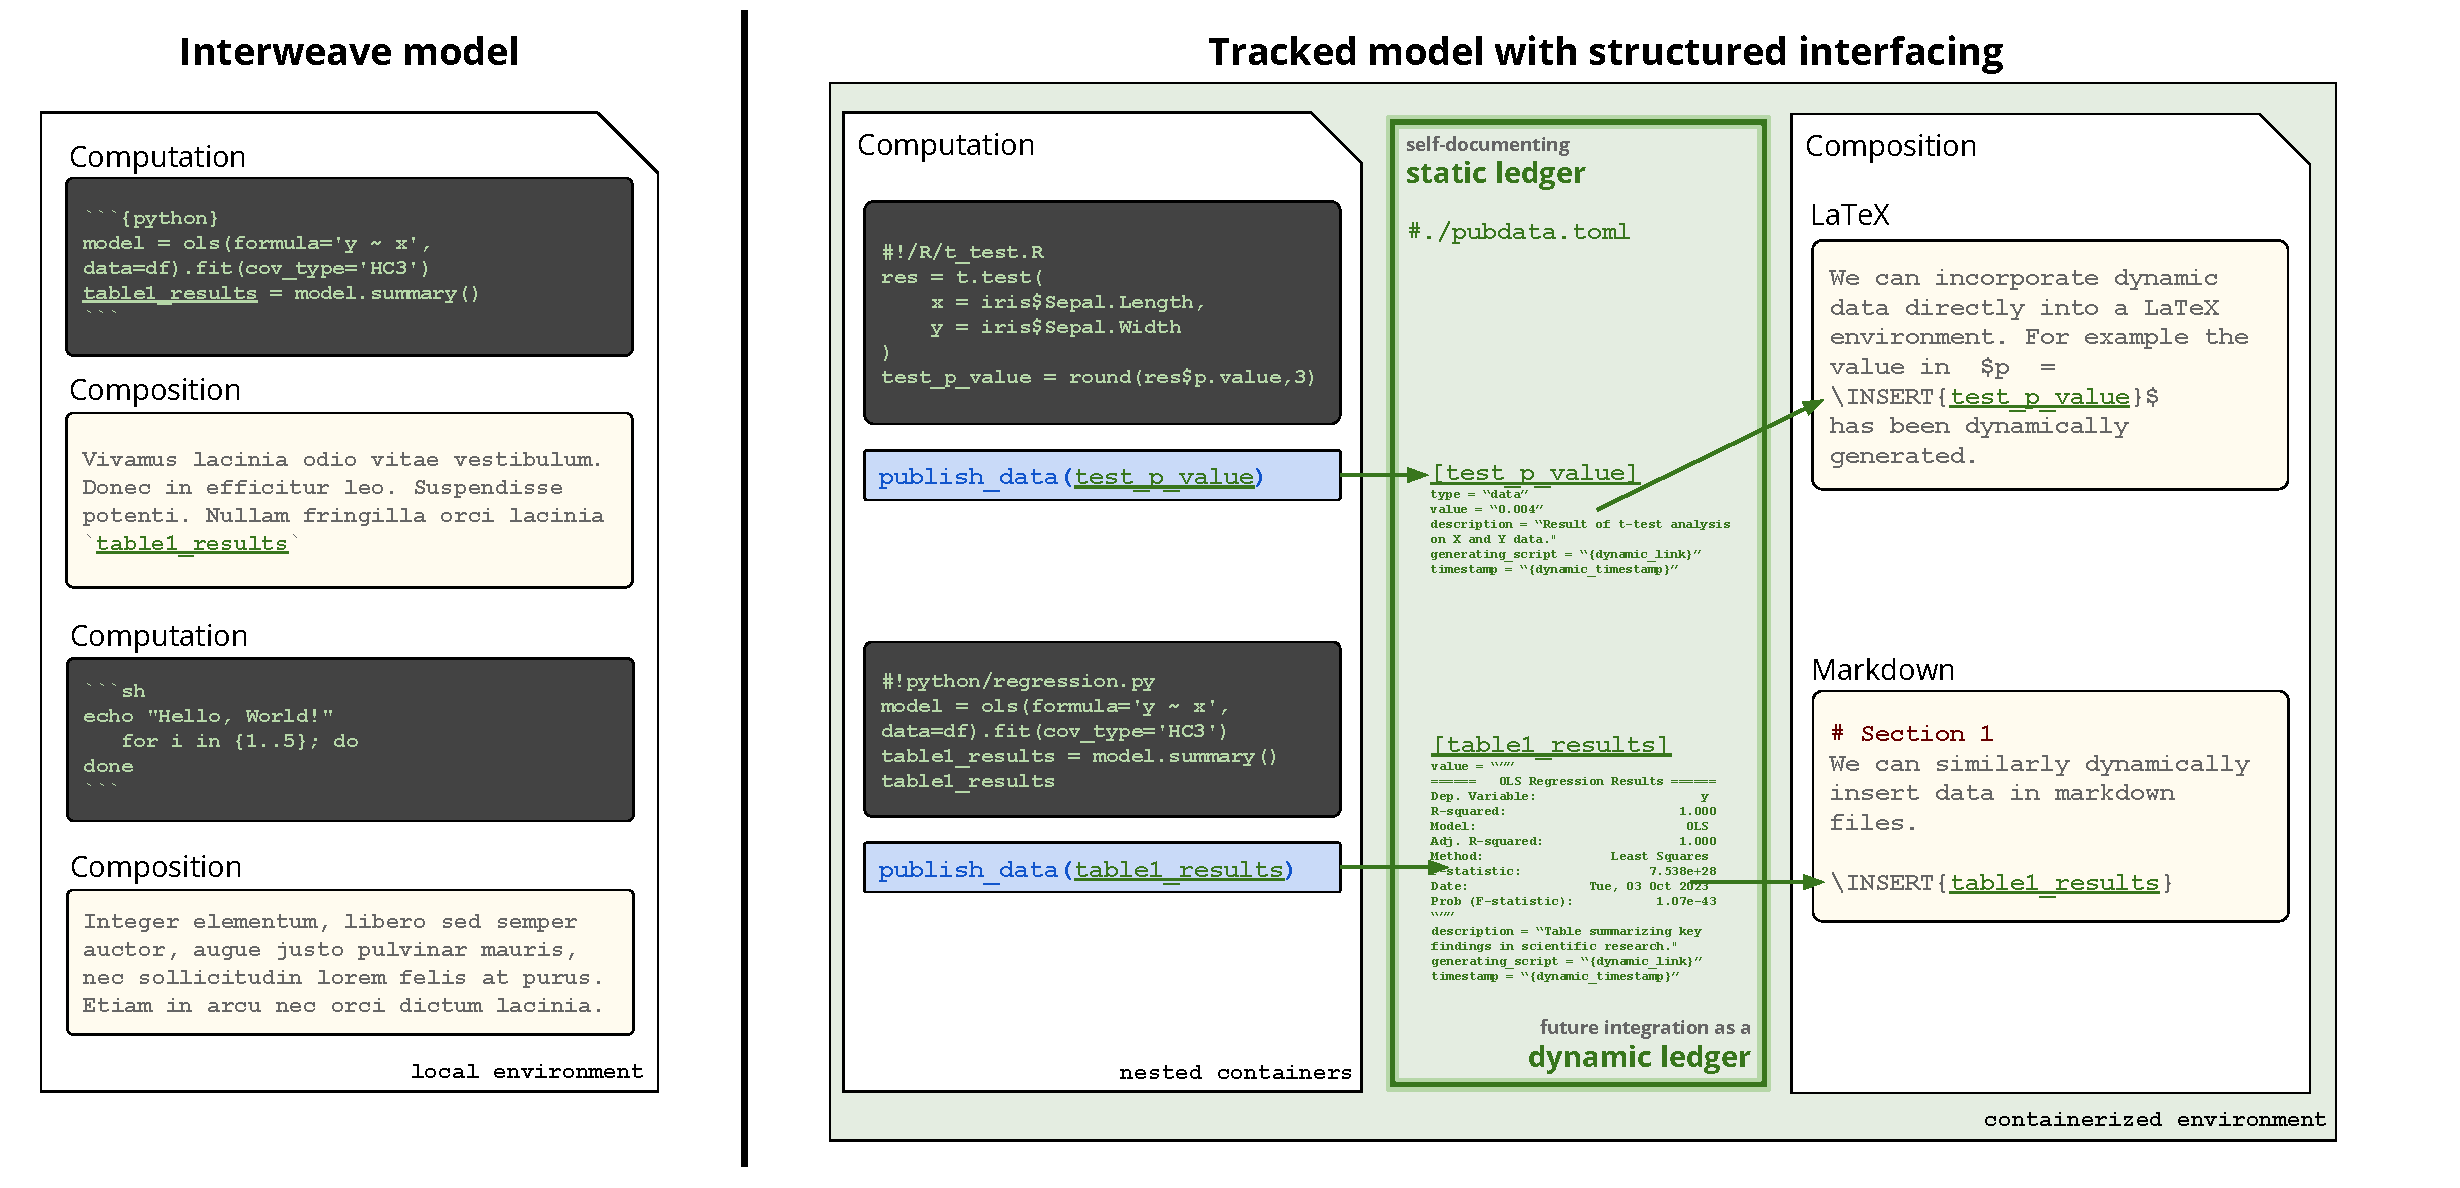
\includegraphics[width=\textwidth]{../../nbs/img/comp.pdf}

\vspace{2mm}
\begin{minipage}{0.95\textwidth}
%\centering
\setstretch{1}
\footnotesize{
\emph{Note:} The \textbf{interweave} model is one in which computation and composition happen linearly within the flow of a single document. Of course, existing paradigms can be quite flexible and allow for a variety of workflows; however, we believe most existing software follows this model. This leads to our proposal of the \textbf{tracked model with structured interfacing}. In this model, the data and code are tracked in a way that allows for easy verification and traceability of reported scientific results with structured metadata.
}
\end{minipage}
\end{figure}



\hypertarget{core-concept-of-the-reproduce.work-framework}{%
\subsection{Core concept of the reproduce.work framework}\label{core-concept-of-the-reproduce.work-framework}}

At the heart of the reproduce.work ecosystem is a commitment to value of structured metadata. The core concept of the reproduce.work framework is that scientific reports should be published with structured metadata that allows for the verification of computational reproducibility. This is a simple idea, but it has profound implications for the way that scientific reports are produced and published.

The main pieces of metadata in our v0.0.1 standards framework include the following:

\begin{itemize}
\itemsep -0.2em
\item \texttt{config.toml}: A configuration file that specifies the computing environment and the software dependencies required to run the code.
\item \texttt{pubdata.toml}: A configuration file that specifies the data used in the report and the code that was used to produce the results.
\end{itemize}

The concept is visualized partiall in Figure \ref{fig:comp}. In this diagram, we try to accomplish several goals. One is to draw the distinction between existing paradigms for all-in-one scientific computing and the \texttt{reproduce.work} model, which, as mentioned, is fundamentally based on its structured metadata. Documents produced with the \texttt{reproduce.work} development kit will automatically generate metadata at the time of computation and publication, with very little overhead to the academic or scientific researcher. This metadata can then be used to verify that the results reported in the published document are indeed reproducible.

As an example, we have included some simulated data and published the metadata and links to the associated code that was used to generate each piece of data. This data has been visuzlied in Figure \ref{fig:scatter}.


\begin{figure}[h]
\centering
\begin{minipage}{0.75\textwidth}
\centering
\caption{A scatter plot generated using Python and compiled into this report using \texttt{reproduce.work} software}
\label{fig:scatter}
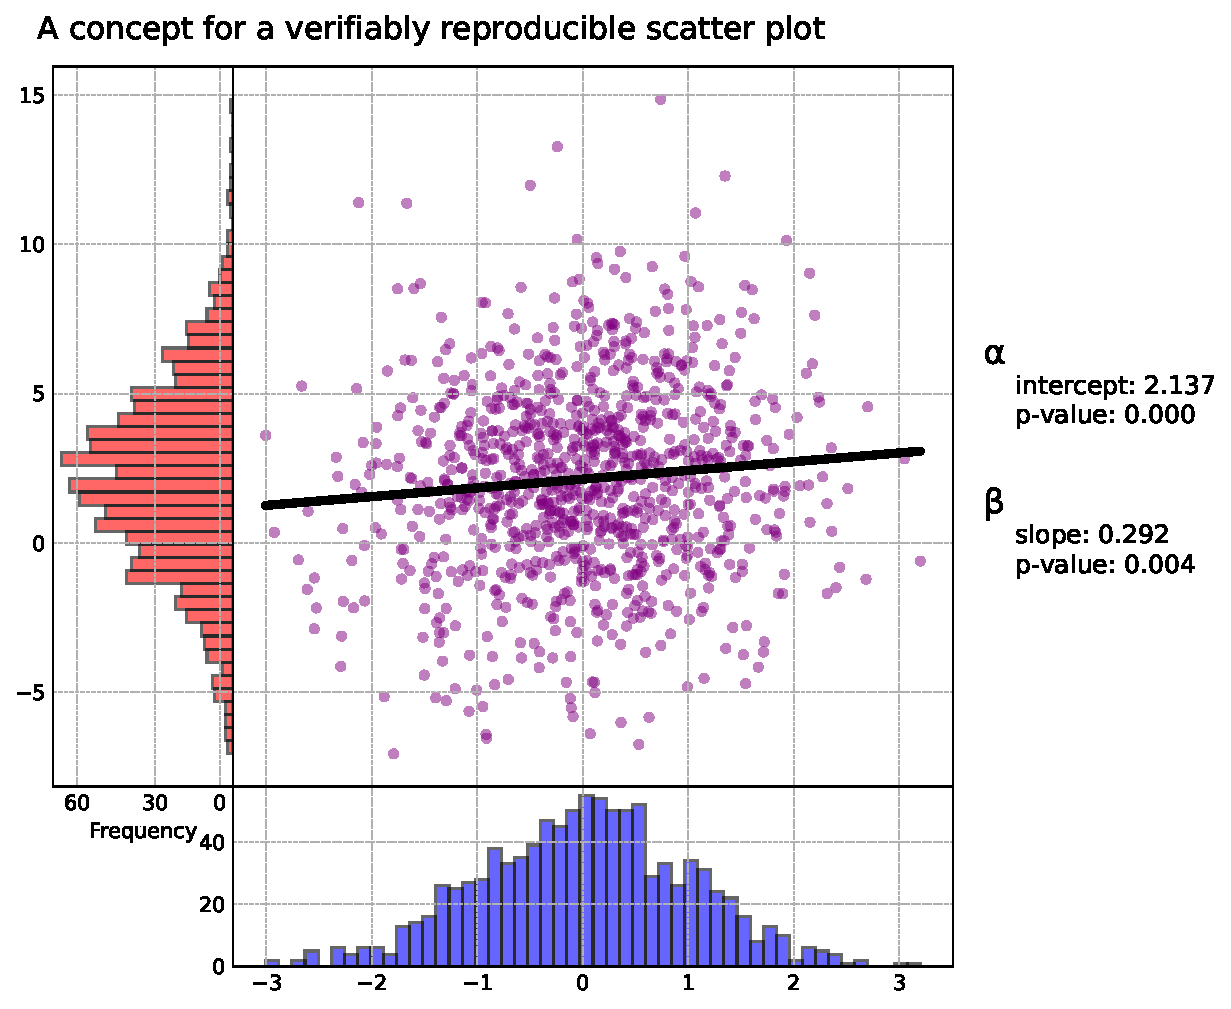
\includegraphics[width=\textwidth]{../../nbs/img/scatter_plot.pdf}

\hfill {\footnotesize \href{https://example.com}{\texttt{open data} \raisebox{-1mm}{
\includegraphics[width=5mm]{../../nbs/img/logo.png}} }} \hspace{-1.5mm}$\;$
\end{minipage}
\end{figure}



We also include dynamic results from the output of statistical code as well, which has been embedded into this document in a way that facilitates tracing of its metadata and generating code. 

\hypertarget{software}{%
\section{Software}\label{software}}

\hypertarget{what-automated-reproducibility-and-verifications-standards-do-for-science}{%
\subsection{What automated reproducibility and verifications standards do for science}\label{what-automated-reproducibility-and-verifications-standards-do-for-science}}

We believe there is some potential for software to address some of the challenges facing science today. In this section we discuss some of the potential benefits and pitfalls of the software put forward in this project, recognizing the inevitable tradeoffs that come with any software design and the complexities that come with the depth and heterogeneity of scientific research.

\hypertarget{what-reproducibility-framework-provides-in-best-case-scenarios}{%
\subsubsection{What reproducibility framework provides in best-case scenarios:}\label{what-reproducibility-framework-provides-in-best-case-scenarios}}

\begin{itemize}
\itemsep -0.2em
\item Transparency: The model ensures that the results presented in a scientific report can be traced back to the source data and the exact processes used to derive them. This transparency can boost confidence in the results.
\item Reproducibility: By encapsulating the environment in Docker and ensuring that the report can be regenerated from the source data and code, the model ensures that results can be reproduced consistently. This is a fundamental aspect of the scientific process.
\item Auditability: With transparency comes the ability to audit. Anyone can inspect the data, code, and environment to ensure that the results have been derived correctly.
\item Modularity: Your design is modular in nature, allowing different build systems and different data input methods. This ensures adaptability across various scientific domains.
\item Standardization: By defining a standard for reproducibility, you're encouraging the scientific community to adhere to a common set of best practices. This can simplify peer reviews and collaborations.
\item Automation: Automated verification reduces human error and ensures consistency in the verification process.
\end{itemize}

\hypertarget{potential-abuses-and-concerns}{%
\subsubsection{Potential Abuses and Concerns:}\label{potential-abuses-and-concerns}}

\begin{itemize}
\itemsep -0.2em
\item False Sense of Security: Just because a report is reproducible doesn't mean it's correct. There might be errors in the data or the methodology. This system verifies reproducibility, not validity.
Tampering with Source Data: If someone manipulates the source data (pubdata.toml or any other input data), they could produce misleading but reproducible results.
\item Over-reliance on Automation: Automated systems can be gamed. For example, someone might find a way to produce the correct hash without following the correct scientific process.
\item Opaque Docker Images: While Docker ensures consistency, it can also hide details. A malicious actor could embed malicious code or data inside a Docker image.
\end{itemize}

Your reproducibility framework offers a robust way to ensure that scientific results can be consistently reproduced, adding a layer of trust and transparency to the process. However, like any system, it's essential to be aware of its potential for misuse and to implement checks and balances. Continuous review and adaptation of the framework, combined with education around its correct use and limitations, can mitigate many of these concerns.

\hypertarget{seemless-reproducible-scientific-computing-via-containerization}{%
\subsection{Seemless reproducible scientific computing via containerization}\label{seemless-reproducible-scientific-computing-via-containerization}}

Scientific computing is very much like other computing, so it should come as no surprise that tools that have been developed to faciltate the reproduction of arbitrary computing tasks can be adapted to the ends of scientists. Containerization is a technology that allows for the creation of self-contained computing ``containers'' that can be run on any computer with the containerization software installed. While this does necessitate the installation of the containerization software, this is a one-time task that can be done by anyone with a computer. Once the containerization software is installed, the promise of containerization is that a container can be run on any computer, regardless of the operating system or other software installed on the computer. Many containerization standards exist; 

\hypertarget{containerization-via-docker}{%
\subsubsection{Containerization via Docker}\label{containerization-via-docker}}

In its current incarnation, we rely on the \href{https://www.docker.com/}{Docker} standard to facilitate cross-platform reproducibility. Docker is a containerization platform that allows for the creation of self-contained computing ``containers'' that can be run on any computer with the containerization software installed. While this does necessitate the installation of the containerization software, this is a one-time task that can be done by anyone with a computer. Once the containerization software is installed, the promise of containerization is that a container can be run on any computer, regardless of the operating system or other software installed on the computer.

It seems possible we could generalize the containerization framework to be more agnostic to the specific containerization standard. However, for the time being, we have chosen to focus on the Docker standard because it is a widely adopted and supported containerization standard, and the standards we aim to clear first is feasibility of replication; in future versions hope to include universal software support (to the degree that it makes sense for the aims of this project). 

\hypertarget{future-directions}{%
\section{Future directions}\label{future-directions}}

In this section we mention some of the ambitious and yet under-developed ideas for future directions for this project.

\hypertarget{data-verification}{%
\subsection{Data verification}\label{data-verification}}

Using reproduce.work structured metadata, we believe there is a possibility to offer some basic forms of data verification that may be of interest to data providers and researchers wishing to signal the independence of their data collection process. Not all scientific reports are amenable to this type of verification, but we believe that many --- particularly those based on human participant data --- are.

In the future, it may be possible for data providers to verify certain aspects of the metadata (including content hashes) that is used by the authors of a scientific report. This would allow for authors to signal some degree of independence around the data collection process. If authors are forced to commit their analysis code to be run only on verified data from a third-party provider (e.g., a university lab or Qualtrics or CloudResearch), then this would allow authors to ``prove'' that key aspects of their analysis plan were committed to before the data were collected. This would be a step toward ensuring that the data used in scientific reports is trustworthy.
We believe the reproduce.work suite of software and standards could play a key role in facilitating this type of verification.

\hypertarget{reproducibility-with-pre-registration-and-order-of-computation}{%
\subsection{Reproducibility with pre-registration and order-of-computation}\label{reproducibility-with-pre-registration-and-order-of-computation}}

There may be value in the ability to pre-register code that is to be executed at a later date. This would allow for the verification of the order-of-computation, which may be of interest to researchers wishing to strongly signal the independence between their data collection process and their analysis plan.

$$ \text{pre-registered code} \rightarrow \text{timestamped data collection} \rightarrow \text{code execution} \rightarrow \text{verified results} $$

There are many details that remain to be worked out, particular which parties would be interested in this type of verification and who would be responsible for its implementation and authentication.
As a simple potential application, we highlight how adversarial collaborations may greatly benefit from such software. The ability to agree on code and data structure and analysis plan prior to data collection might facilitate a new form of collaborations between parties that may otherwise have opposing views --- enabled by the ability to verify the order-of-computation. Having a set of standards and rules by which different parties agree to abide will be key to ensure such collaborations are independently verifiable and reproducible.  It seems possible the reproduce.work suite of software and standards could play a key role in facilitating this type of verification.

\hypertarget{leveraging-language-models-for-enhanced-automated-forms-of-verification}{%
\subsection{Leveraging language models for enhanced, automated forms of verification}\label{leveraging-language-models-for-enhanced-automated-forms-of-verification}}

The capabilities of language models open up potential for new and heretofore exotic forms of automated verification. 
A simple example of this is the ability to ``read'' the content of a final scientific document to identify every reported statistic and piece of data that is referenced in the manuscript. We can then take these entities and cross-reference them with the open data entry in the project's structured metadata. We can then ensure that the data and code provided by the authors of the document can be executed to produce the data that was published and the same output as the final document.

Further scenarios may involve using language models to provide automated summaries of statistical derivations. In theory, so long as all the code is indeed open, one can imagine using a chain-of-thought language model to trace the derivation of a statistical result from the data, through the logic of the code, to the final result in the manuscript. Though perhaps not strictly ``verification'', such processes may enhance the generation of better metadata and documentation of scientific results. The ability of language models to summarize human-readable text also has the potential to significantly improve the comprehensibility and readability of scientific papers. There may be great potential for facilitating various forms of review in the scientific publishing process --- including automated, peer, or both --- using language models.

\hypertarget{conclusion}{%
\section{Conclusion}\label{conclusion}}

One may ask whether the framework here prevents questionable research practices including undesirable behavior like $p$-hacking or seed hacking. Unfortunately, the framework put forward here is not a panacea. The bar we set out to clear in this version of the project was to take steps toward a world where computational reproduction is possible. Developing software specifically designed to discourage bad or encourage good aspects of research behavior is a task for future work. Nonetheless, it is valuable to discuss some ideas in which we may use our computing paradigm to encourage certain behaviors and practices of quantitative research.

One such method for exploration in future versions of this work is the potential for pre-registering exactly the model specification with which one wishes to estimate. If we were forced to pre-register our exact model specifications, we would be discouraged from pursuing models that depend on researcher degrees of freedom that can be exploited between the collection of data and reporting of results. As such, this may encourage scientists to explore the use of machine learning for analysis of heterogeneous treatment effects or specification curve analyses that are designed to be robust to specification searching. 

The project put forward in the body of this project is a mere first step in the direction of computational reproduction. The software lacks support for many important features and the concept is heretofore untested. While there are many aspects to reproducibility in the epistemology of science, we believe that computational reproducibility is a necessary first step toward a world where scientific results are verifiable and trustworthy. However, given the low bars required to improve the existing practices around computational reproduction, we beleive this project and the ideas put forward here have potential as the seed of a growing culture of scientific rigor and transparency.
\bibliography{bibliography}\end{document}